\documentclass[conference]{IEEEtran}
% \IEEEoverridecommandlockouts   % uncomment only if \thanks is needed
\usepackage{cite}
\usepackage{amsmath,amssymb,amsfonts}
\usepackage{algorithmic}
\usepackage{graphicx}
\usepackage{textcomp}
\usepackage{xcolor}
\usepackage{url}
\interdisplaylinepenalty=2500

% Template: ../LASCAS/PAPER_LASCAS_2027_SNP-AV1_SUBMIT.tex
% Binding decisions and pre-registration: ISCAS/CLAUDE.md
% Every BD-BR and TS value comes from the CTC Class A1 grid only.

\begin{document}

\title{NPL-AV1: A Neural Pruner Ladder for the AV1\\ Intra-Frame Partition Search}

\author{
\IEEEauthorblockN{
Pablo Rosa,
Daniel Palomino,
Marcelo Porto,
Luciano Agostini
}
\IEEEauthorblockA{
\textit{Video Technology Research Group (ViTech)}\\
\textit{Federal University of Pelotas}\\
Pelotas, Brazil\\
\{pablo.rosa, dpalomino, porto, agostini\}@inf.ufpel.edu.br
}
}

\maketitle

\begin{abstract}
The intra-frame coding of the AOMedia Video 1 (AV1) codec selects the block
partitioning through a recursive rate-distortion search, and its reference
encoder already embeds a convolutional neural network that prunes this search at
the fast speed presets. Fast partitioning solutions are usually compared against
whole presets, which reconfigure every other coding stage as well, so the
contribution of a neural pruner itself is not measured. This paper presents the
Neural Pruner Ladder for AV1 (NPL-AV1), a set of shallow neural networks that
replace the native network as partition pruners at the same speed preset. A
pre-search pruner removes partition types before any rate-distortion
evaluation, and a post-NONE pruner decides whether the search
continues after the unpartitioned node is measured, a decision that no neural
model of the native encoder takes in All-Intra coding. Experimental results over
the eight UHD 4K sequences of the AOM Common Test Conditions show that the
post-NONE pruner achieves time savings of 30.34\% with a Bjontegaard delta
bitrate (BD-BR) of 0.41\% at preset 1, with no statistically significant BD-BR
difference from the native network at presets 1 and 2, a significantly lower
BD-BR at high quality at both presets, and a higher BD-BR at preset 3. The
pre-search pruner extends the time savings of each preset up to 77.30\%, at a
BD-BR of 4.35\%. % [completar: fracao de pontos nao dominados de NPL-AV1, recalculada com tau_stop=0.95 apenas e com os pontos da campanha D2 (sem D2: 9 de 12)]
% [completar: frase do H9d empilhado, apos a campanha D2]
To the best of the authors' knowledge, this is the first solution in the
literature measured as a replacement of the native partition network of AV1.
\end{abstract}

\begin{IEEEkeywords}
Video coding, AV1, computational effort reduction, intra-frame block
partitioning, neural networks, encoder speed presets.
\end{IEEEkeywords}

% ---------------------------------------------------------------------------
% Body: written block by block (ISCAS/CLAUDE.md, section 3).
% I.   Introduction
% II.  The AV1 Intra-Frame Partition Search
% III. Proposed NPL-AV1 Solution
% IV.  Results and Comparisons
% V.   Conclusions
% ---------------------------------------------------------------------------

\section{Introduction}
\label{sec_intro}

The number of Internet users watching online video every month keeps growing
\cite{statista}. The AOMedia Video 1 (AV1) was released in 2018 by the Alliance
for Open Media (AOMedia) \cite{av1site}, alongside the High Efficiency Video
Coding (HEVC) \cite{hevc} and the Versatile Video Coding (VVC) \cite{vvc}, from
the ITU-T Video Coding Experts Group and the ISO/IEC Moving Picture Experts
Group. Each step of its hybrid coding flow, from prediction to entropy
coding, introduces new techniques \cite{han2021,chen2018}. Its coding efficiency
is superior to that of HEVC under certain conditions \cite{grois2016}, at the
price of encoding times about twice as long \cite{layek2017}.

The processing of the partition tree is one of the large computational costs of
the AV1 reference encoder \cite{bender2023}. Each superblock is divided by a
recursive search that evaluates up to ten partition types per node through
rate-distortion optimization (RDO) \cite{sullivan1998}. The reference software
libaom \cite{libaom} performs this search in full at \texttt{cpu-used=0} and
prunes it at the fast presets. From \texttt{cpu-used=1} on, its All-Intra configuration
enables the \texttt{intra\_cnn\_based\_part\_prune} speed feature \cite{libaom},
a convolutional neural network (CNN) that reads each 64$\times$64 block once and, before any RDO, forces or forbids the quad-tree split down to
8$\times$8 samples. A preset also changes the transform, intra mode and loop
filter searches, so a solution compared against a preset is measured against
every speed feature at once, not against the partition pruner alone.

Few works act on the computational effort of AV1. None of them acts on the
partition network of its reference encoder. The works \cite{xu2020,xu2021,jeong2019} reduce
the intra prediction mode decision, \cite{kim2019} applies decision trees to
inter prediction, and \cite{correa2020,netto2022} are hardware designs for the
intra predictor rather than for encoder decisions. Neural partition prediction
was integrated into the VP9 encoder through a hierarchical CNN \cite{paul2020},
and learning-based partitioning solutions exist for VVC, through variance and
gradients, random forests and gradient boosting, texture complexity, or the
regression of RD costs
\cite{chen2019,he2021,saldanha2022,song2024,kherchouche2024,kherchouche2025}, but
they were designed for the partition structures of those codecs and evaluated on
their encoders, which prevents a direct and fair comparison. The contribution of
a neural pruner against the native network, at the same preset, is therefore not
measured.

This paper presents the Neural Pruner Ladder for AV1 (NPL-AV1), a set of shallow
multilayer perceptrons (MLPs) that replace the native CNN in the libaom
intra-frame partition search. The main strategy of this solution is to consult
each pruner where the information it reads already exists, and to measure it at
a fixed preset with the native network disabled, so only the partition pruner
changes. A pre-search pruner reads the content and the causal partition context
of the node before any RDO. A post-NONE pruner also reads the RD cost of the
unpartitioned node and decides whether the search continues, a decision that no
neural model of the native encoder takes in All-Intra coding. Over the eight UHD
4K sequences of the AOM Common Test Conditions (CTC), the post-NONE pruner shows
no statistically significant difference in coding efficiency from the native CNN
at presets 1 and 2 and a significantly lower coding efficiency loss at high
quality, while the pre-search pruner extends the time savings of every preset,
so each preset has three operating points instead of one.

\section{The AV1 Intra-Frame Partition Search}
\label{sec_search}

The basic unit of AV1 partitioning is the superblock, of 128$\times$128 or
64$\times$64 samples, which the partition tree divides recursively down to
4$\times$4 samples \cite{han2021}. Each node may take one of ten partition types
\cite{chen2018}: NONE codes the node as a single block, SPLIT divides it into four
square sub-blocks, HORZ and VERT divide it into two rectangular sub-blocks, the
four AB types join a rectangular half to two square sub-blocks, and the two 4-way
types divide it into four sub-blocks of 4:1 aspect ratio. Together, the AB and
4-way families are the extended partitions.

The libaom encoder evaluates the types of a node in a fixed order, NONE, SPLIT, the
rectangular and then the extended types \cite{libaom}, so what a pruner can read
depends on where it is consulted. Before NONE, only the samples, the quantization
and the decisions of the already coded neighbors exist; after NONE, the rate, the
distortion and the RD cost of the unpartitioned node exist as well, at the price
of having been paid.

The native neural pruners act at both points, but not with the same reach in
All-Intra coding. Before the search, the CNN of Section~\ref{sec_intro} forces or
forbids the split from \texttt{cpu-used=1} on. After NONE, three neural decisions
can end the search of the node or remove candidates from it: a breakout after NONE, an early
termination after SPLIT and the pruning of the rectangular types. All three are
disabled in intra-only frames by a frame-type guard \cite{libaom}, while two other
networks stay active and prune the AB and 4-way types from the RD costs already
measured. Whether the search of a node continues once its unpartitioned cost is
known is, therefore, a decision that no neural model of the native encoder takes
in All-Intra coding.

This work is focused on the intra-frame partition search of AV1 under the
All-Intra (AI) configuration. The intra prediction modes, the transform type and
the loop filters are decided inside each evaluated partition type, not by the
partition search itself, and therefore they are not focused on this work, nor is
the inter-frame partition search.

\section{Proposed NPL-AV1 Solution}
\label{sec_method}

The Neural Pruner Ladder for AV1 (NPL-AV1) inserts MLP pruners at the two points
of the node search identified in Section~\ref{sec_search}, as shown in
Fig.~\ref{fig_npl}. The main strategy of this solution is to give each preset of
libaom a choice of partition pruner instead of a single one: with the native CNN
disabled, a pre-search or a post-NONE pruner replaces it, and every other speed
feature of the preset is kept as it is.

\begin{figure}[!t]
  \centering
  % src/scripts/benchmark/plot_npl_ladder_iscas_fig1.py (variante cinza)
  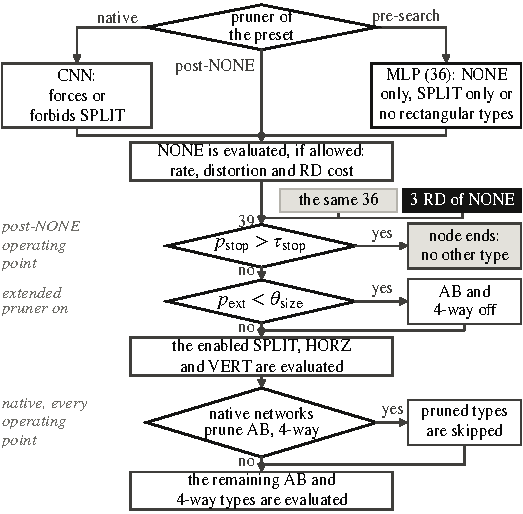
\includegraphics[width=\columnwidth]{fig1_npl_ladder}
  \caption{NPL-AV1 flowchart for one node at a fixed preset. The operating
  point of the preset selects the pruner that acts before the search, the post-NONE and
  extended pruners act after NONE is evaluated, and the shaded action ends the node.}
  \label{fig_npl}
\end{figure}

The pre-search pruner is consulted where the native CNN is and acts on the same
structural axis: it may settle the node as NONE and cut the whole subtree below
it, commit the node to SPLIT, or remove the rectangular types and, with them, the
extended ones. The post-NONE and the extended pruners are consulted after NONE has
been evaluated, the point at which the three structural decisions of the native
encoder are disabled in All-Intra coding. The post-NONE pruner decides whether
the search of the node ends there, and the extended pruner whether the AB and
4-way types are worth evaluating, the only decision that the native networks
still take after NONE. Every pruner only removes candidates, so moving between
the operating points of a preset is a matter of choosing which pruner replaces
the CNN, not of retraining it.

\subsection{Features, Dataset and Models}
\label{sec_models}

Every pruner reads features whose extraction demands no rate-distortion
evaluation of its own. Twenty-four block-content features (BC) are statistics of
the samples of the node, of its quadrants and of its contrast with the parent and
sibling sub-blocks, together with the quantization and the position of the node;
eight causal-neighbor partition context features (NC) read the partition of the
coded blocks above and on the left; and four coding-state and position features
(CSP) are added to them, for thirty-six features in the pre-search pruner. The
post-NONE and the extended pruners also read the logarithms of the rate, the
distortion and the RD cost of the measured NONE.

The label of every node comes from an extraction with libaom v3.10.0,
instrumented to record the decision of the encoder with these features at
\texttt{cpu-used=0}, since only an exhaustive search gives a faithful label. All
sixteen UHD 4K sequences of UVG \cite{uvg} were encoded over five frames at
\texttt{cq-level} 20, 32, 43 and 55, with ten sequences kept for training, three
for validation and three for testing. The CTC sequences of
Section~\ref{sec_results} do not belong to UVG, which rules out data leakage
between training, testing and evaluation.

Every pruner is a set of three MLPs, for nodes of 16, 32 and 64 samples, whose
two hidden layers have 64 and 32 ReLU units. The pre-search and the post-NONE
pruners give the probabilities of NONE, of SPLIT and of the remaining types, and
the extended pruner gives the probability $p_{\mathrm{ext}}$ that the best type
of the node is an extended one. The models were trained over 30 epochs under
hard-label cross entropy, with the AdamW optimizer \cite{adamw} in PyTorch
\cite{pytorch}, and the standardization of the features was folded into the
first layer, so the encoder executes the models over raw features.

\subsection{Decision Rules and Encoder Integration}
\label{sec_policy}

The pre-search pruner reads its probabilities in a fixed order: the node is
settled as NONE, with the whole subtree below it cut, when
$p_{\mathrm{none}} > \tau_{\mathrm{none}}$; otherwise it is committed to SPLIT
when $p_{\mathrm{split}} > \tau_{\mathrm{split}}$; otherwise its rectangular
types are disabled, together with the extended ones, when
$p_{\mathrm{rest}} < \tau_{\mathrm{rest}}$. The post-NONE pruner ends the search
of the node when its probability of NONE, $p_{\mathrm{stop}}$, exceeds
$\tau_{\mathrm{stop}} = 0.95$, and the extended pruner disables the AB and 4-way
types when $p_{\mathrm{ext}} < \theta_{\mathrm{size}}$, with
$\theta_{\mathrm{size}} = 0.0910$ for nodes of 16 samples, 0.1031 for 32 and
0.0144 for 64.

A higher $\tau_{\mathrm{none}}$ or $\tau_{\mathrm{split}}$, or a lower
$\tau_{\mathrm{rest}}$, demands more confidence from the model before a candidate
is removed, so fewer nodes are pruned, fewer wrong decisions are taken and less
coding efficiency is lost, at the price of smaller time savings; loosening the
three thresholds moves the pruner the other way. Two operating points were
selected at opposite sides of this trade-off, set by
$(\tau_{\mathrm{none}}, \tau_{\mathrm{split}}, \tau_{\mathrm{rest}})$: the
efficiency-first one, $(0.95, 0.90, 0.20)$, which is stricter in all three
thresholds, and the time-first one, $(0.60, 0.85, 0.40)$, which is looser in all
three. A third one, $(0.90, 0.90)$ with $\tau_{\mathrm{rest}}$ disabled, is only
evaluated at \texttt{cpu-used=0} together with the post-NONE pruner.

All pruners were implemented in C within libaom v3.10.0. With their compile-time
guard disabled, the build gives the bitstream of the reference software byte for
byte, and the native CNN is disabled in the same binary, so at each preset the
partition pruner is the only difference from the native configuration. Since
every pruner removes candidates and never forces one, NPL-AV1 is fully compliant
with the AV1 specification and does not affect the bitstream syntax.

\section{Results and Comparisons}
\label{sec_results}

NPL-AV1 was evaluated in the libaom v3.10.0 reference software under the
All-Intra configuration of the AOM CTC \cite{ctc}, over the eight sequences of
Class A1, of 3840$\times$2160 samples, 10-bit depth and 4:2:0 chroma subsampling
\cite{xipha1}, of which the first 15 frames were encoded at \texttt{cq-level} 20,
32, 43 and 55, with the two-tile setting of the CTC for 4K content, against
libaom at \texttt{cpu-used=0} as anchor. Three deviations from the CTC are
declared: the quantization is set by \texttt{cq-level}, since this version of
libaom has no \texttt{--qp} option; the time is the wall time of each encode;
and the configurations under evaluation run at presets 1, 2 and 3, while only
the anchor keeps \texttt{cpu-used=0}, since the preset is the controlled
variable of this work. The BD-BR \cite{bjontegaard} uses the luma PSNR, and a
positive value is a coding efficiency loss. With $t(s,q)$ and
$t_{\mathrm{anc}}(s,q)$ the encoding times of a configuration and of the anchor
for sequence $s$ at \texttt{cq-level} $q$, and $S$ and $Q$ the sets of sequences
and of \texttt{cq-level} values, the time savings are
\begin{equation}
\mathrm{TS} = \frac{100}{|S|} \sum_{s \in S} \frac{1}{|Q|} \sum_{q \in Q}
\left( 1 - \frac{t(s,q)}{t_{\mathrm{anc}}(s,q)} \right) \%.
\label{eq_ts}
\end{equation}
Each configuration was encoded once. Five repeated encodes on one sequence give
0.23 percentage points of standard deviation for TS, so TS differences under 0.46
points are not resolved; the BD-BR comes from the bitstream size and the PSNR,
which are exact.

Table~\ref{tab_replace} gives both metrics for the native CNN and for the
NPL-AV1 pruners that replace it at each preset. The post-NONE pruner and the
native CNN are comparable at presets 1 and 2: 0.414\% against 0.449\% of BD-BR
at preset 1 and 0.516\% against 0.536\% at preset 2, for 30.34\% and 40.73\% of
TS against 32.59\% and 42.72\%. The paired t-tests of Table~\ref{tab_ttest},
over the eight sequences, show no significant BD-BR difference at either
preset, while the TS of the post-NONE pruner is lower by 2.25 percentage points
at preset 1 ($p = 0.046$) and by 1.99 at preset 2 ($p = 0.055$). At preset 3
the replacement has a BD-BR higher by 0.662 points, in all eight sequences.

\begin{table}[!t]
\renewcommand{\arraystretch}{1.1}
\caption{BD-BR and TS of the Native CNN and of the NPL-AV1 Pruners at the Same
Preset}
\label{tab_replace}
\centering
\setlength{\tabcolsep}{4pt}
\begin{tabular}{lcccccc}
\hline
 & \multicolumn{2}{c}{\textbf{Preset 1}} & \multicolumn{2}{c}{\textbf{Preset 2}}
 & \multicolumn{2}{c}{\textbf{Preset 3}} \\
\textbf{Pruner} & \textbf{BD-BR} & \textbf{TS} & \textbf{BD-BR} & \textbf{TS}
 & \textbf{BD-BR} & \textbf{TS} \\
 & (\%) & (\%) & (\%) & (\%) & (\%) & (\%) \\
\hline
Native CNN & 0.449 & 32.59 & 0.536 & 42.72 & 2.722 & 67.94 \\
Post-NONE & 0.414 & 30.34 & 0.516 & 40.73 & 3.384 & 70.25 \\
\multicolumn{7}{l}{Pre-search:} \\
\quad Efficiency-first & 0.915 & 40.20 & 1.030 & 50.05 & 3.866 & 73.09 \\
\quad\quad + extended$^{\mathrm{a}}$ & 0.947 & 41.15 & 1.069 & 50.99 & 3.868 & 72.96 \\
\quad Time-first & 1.685 & 51.82 & 1.805 & 60.97 & 4.347 & 77.30 \\
\hline
\multicolumn{7}{l}{\footnotesize $^{\mathrm{a}}$With the extended pruner; separate campaign, increment}\\
\multicolumn{7}{l}{\footnotesize \phantom{$^{\mathrm{a}}$}measured over a re-encoded base and discussed below.}
\end{tabular}
\end{table}

\begin{table}[!t]
\renewcommand{\arraystretch}{1.1}
\caption{Paired t-Tests of the Post-NONE Pruner Against the Native CNN, Over
Eight Sequences}
\label{tab_ttest}
\centering
\begin{tabular}{cccccc}
\hline
\textbf{Preset} & \textbf{cq-level} & \textbf{$\Delta$BD-BR} & \textbf{$p$}
 & \textbf{$\Delta$TS} & \textbf{$p$} \\
 & & (pp) & & (pp) & \\
\hline
1 & all & $-0.034$ & 0.278 & $-2.25$ & 0.046 \\
1 & 20, 32 & $-0.088$ & 0.043 & $-4.29$ & 0.036 \\
1 & 43, 55 & $+0.009$ & 0.826 & $-0.22$ & 0.678 \\
2 & all & $-0.020$ & 0.291 & $-1.99$ & 0.055 \\
2 & 20, 32 & $-0.086$ & 0.015 & $-3.88$ & 0.041 \\
2 & 43, 55 & $+0.027$ & 0.467 & $-0.10$ & 0.859 \\
3 & all & $+0.662$ & 0.004 & $+2.30$ & 0.002 \\
\hline
\end{tabular}
\end{table}

The average over the whole grid is the mean of two different regimes. At
\texttt{cq-level} 20 and 32, the post-NONE pruner lowers the BD-BR of the native
CNN by 0.088 points at preset 1 and by 0.086 at preset 2, both significant
($p = 0.043$ and $p = 0.015$) and in six and seven of the eight sequences, at a
cost of 4.29 and 3.88 percentage points of TS. At \texttt{cq-level} 43 and 55
the two pruners do not differ in BD-BR. This split by quantization regime was
made after the result over the whole grid and is not corrected for multiple
comparisons; its support is the replication of the same sign and magnitude at
two independent presets. This fact partly explains why a shallow model reaches
the coding efficiency of the native network: it reads the measured RD cost of
NONE, which no neural model of the native encoder reads before deciding whether
the search of the node continues.

\section*{Acknowledgment}

This study was financed in part by the Coordena\c{c}\~ao de Aperfei\c{c}oamento de
Pessoal de N\'ivel Superior -- Brasil (CAPES) -- Finance Code 001, and also by the
Brazilian research support agencies CNPq and FAPERGS.

% \IEEEtriggeratref{n}  % set only when the last page needs balancing
\begin{thebibliography}{00}

\bibitem{statista} Statista. (2025). \emph{Share of Internet Users Watching Online Videos Every Month From 1st Quarter 2022 to 3rd Quarter 2024}. [Online]. Available: \url{https://www.statista.com/statistics/1489445/online-video-viewers-worldwide-quarterly/}

\bibitem{av1site} Alliance for Open Media. (2019). \emph{AV1 Video Codec}. [Online]. Available: \url{https://aomedia.org/av1}

\bibitem{hevc} ITU-T. (2013). \emph{H.265: High Efficiency Video Coding}. [Online]. Available: \url{https://www.itu.int/rec/t-rec-h.265}

\bibitem{vvc} ITU-T. (2020). \emph{H.266: Versatile Video Coding}. [Online]. Available: \url{https://www.itu.int/rec/t-rec-h.266}

\bibitem{han2021} J. Han \emph{et al.}, ``A technical overview of AV1,'' \emph{Proc. IEEE}, vol. 109, no. 9, pp. 1435--1462, Sep. 2021.

\bibitem{chen2018} Y. Chen \emph{et al.}, ``An overview of core coding tools in the AV1 video codec,'' in \emph{Proc. Picture Coding Symp. (PCS)}, Jun. 2018, pp. 41--45.

\bibitem{grois2016} D. Grois, T. Nguyen, and D. Marpe, ``Coding efficiency comparison of AV1/VP9, H.265/MPEG-HEVC, and H.264/MPEG-AVC encoders,'' in \emph{Proc. Picture Coding Symp. (PCS)}, Dec. 2016, pp. 1--5.

\bibitem{layek2017} M. A. Layek \emph{et al.}, ``Performance analysis of H.264, H.265, VP9 and AV1 video encoders,'' in \emph{Proc. 19th Asia-Pacific Netw. Oper. Manage. Symp. (APNOMS)}, Sep. 2017, pp. 322--325.

\bibitem{bender2023} I. Bender \emph{et al.}, ``Complexity and compression efficiency analysis of libaom AV1 video codec,'' \emph{J. Real-Time Image Process.}, vol. 20, no. 3, art. no. 50, May 2023.

\bibitem{sullivan1998} G. J. Sullivan and T. Wiegand, ``Rate-distortion optimization for video compression,'' \emph{IEEE Signal Process. Mag.}, vol. 15, no. 6, pp. 74--90, Nov. 1998.

\bibitem{libaom} Alliance for Open Media. \emph{AV1 Codec Library}, v3.10.0. [Online]. Available: \url{https://aomedia.googlesource.com/aom}

\bibitem{xu2020} M. Xu and B. Jeon, ``Selection of intra prediction tools for fast AV1 encoding,'' in \emph{Proc. IEEE Int. Symp. Broadband Multimedia Syst. Broadcast. (BMSB)}, Oct. 2020, pp. 1--4.

\bibitem{xu2021} M. Xu and B. Jeon, ``User-priority based AV1 coding tool selection,'' \emph{IEEE Trans. Broadcast.}, vol. 67, no. 3, pp. 736--745, Sep. 2021.

\bibitem{jeong2019} J. Jeong, G. Gankhuyag, and Y.-H. Kim, ``A fast intra mode decision based on accuracy of rate distortion model for AV1 intra encoding,'' in \emph{Proc. 34th Int. Tech. Conf. Circuits/Syst., Comput. Commun. (ITC-CSCC)}, Jun. 2019, pp. 1--3.

\bibitem{kim2019} J. Kim, S. Blasi, A. S. Dias, M. Mrak, and E. Izquierdo, ``Fast inter-prediction based on decision trees for AV1 encoding,'' in \emph{Proc. IEEE Int. Conf. Acoust., Speech Signal Process. (ICASSP)}, May 2019, pp. 1627--1631.

\bibitem{correa2020} M. M. Corr\^ea \emph{et al.}, ``A high-throughput hardware architecture for AV1 non-directional intra modes,'' \emph{IEEE Trans. Circuits Syst. I, Reg. Papers}, vol. 67, no. 5, pp. 1481--1494, May 2020.

\bibitem{netto2022} L. Neto, M. Corr\^ea, D. Palomino, L. Agostini, and G. Corr\^ea, ``Power-quality configurable hardware design for AV1 directional intraframe prediction,'' \emph{IEEE Des. Test}, vol. 39, no. 2, pp. 38--45, Apr. 2022.

\bibitem{paul2020} S. Paul, A. Norkin, and A. C. Bovik, ``Speeding up VP9 intra encoder with hierarchical deep learning-based partition prediction,'' \emph{IEEE Trans. Image Process.}, vol. 29, pp. 8134--8148, 2020.

\bibitem{chen2019} J. Chen, H. Sun, J. Katto, X. Zeng, and Y. Fan, ``Fast QTMT partition decision algorithm in VVC intra coding based on variance and gradient,'' in \emph{Proc. IEEE Vis. Commun. Image Process. (VCIP)}, Dec. 2019, pp. 1--4.

\bibitem{he2021} Q. He, W. Wu, L. Luo, C. Zhu, and H. Guo, ``Random forest based fast CU partition for VVC intra coding,'' in \emph{Proc. IEEE Int. Symp. Broadband Multimedia Syst. Broadcast. (BMSB)}, Aug. 2021, pp. 1--4.

\bibitem{saldanha2022} M. Saldanha, G. Sanchez, C. Marcon, and L. Agostini, ``Configurable fast block partitioning for VVC intra coding using light gradient boosting machine,'' \emph{IEEE Trans. Circuits Syst. Video Technol.}, vol. 32, no. 6, pp. 3947--3960, Jun. 2022.

\bibitem{song2024} Y. Song, S. Cheng, M. Wang, and X. Peng, ``Fast CU partition for VVC intra-frame coding via texture complexity,'' \emph{IEEE Signal Process. Lett.}, vol. 31, pp. 959--963, 2024.

\bibitem{kherchouche2024} M. E. A. Kherchouche, F. Galpin, T. Dumas, D. Menard, and L. Zhang, ``RD-cost regression speed up technique for VVC intra block partitioning,'' in \emph{Proc. IEEE Int. Conf. Acoust., Speech Signal Process. (ICASSP)}, Apr. 2024, pp. 3530--3534.

\bibitem{kherchouche2025} M. E. A. Kherchouche \emph{et al.}, ``Complexity reduction study based on RD costs approximation for VVC intra partitioning,'' in \emph{Proc. Data Compression Conf. (DCC)}, Mar. 2025, p. 377.

\bibitem{uvg} A. Mercat, M. Viitanen, and J. Vanne, ``UVG dataset: 50/120fps 4K sequences for video codec analysis and development,'' in \emph{Proc. 11th ACM Multimedia Syst. Conf. (MMSys)}, Jun. 2020, pp. 297--302.

\bibitem{adamw} I. Loshchilov and F. Hutter, ``Decoupled weight decay regularization,'' in \emph{Proc. Int. Conf. Learn. Represent. (ICLR)}, May 2019, pp. 1--18.

\bibitem{pytorch} A. Paszke \emph{et al.}, ``PyTorch: An imperative style, high-performance deep learning library,'' in \emph{Proc. Adv. Neural Inf. Process. Syst. (NeurIPS)}, Dec. 2019, pp. 8024--8035.

\bibitem{ctc} X. Zhao \emph{et al.}, ``AOM common test conditions v9.0,'' Alliance for Open Media, Codec Working Group, doc. CWG-G082, Mar. 2026.

\bibitem{xipha1} Xiph.Org Foundation. \emph{AOM CTC Test Set, Class A1 (4K)}. [Online]. Available: \url{https://media.xiph.org/video/aomctc/test_set/a1_4k/}

\bibitem{bjontegaard} G. Bj{\o}ntegaard, ``Calculation of average PSNR differences between RD-curves,'' Video Coding Experts Group (VCEG), doc. VCEG-M33, Mar. 2001.

\end{thebibliography}

\end{document}
